\chapter{Adaptation of Botarellis work to atoms} \label{Chapter4}

\noindent
From the start, it is clear that directional routing as discussed in \autoref{Chapter3} is not possible with atoms.
The open system dynamics lead to an effective Hamiltonian in Eq. \eqref{eq:reduces_H_eff} which is non-Hermitian.
Thus, unlike the system in Chapter 3, a setup with $N$ atoms offers no chirality.
To qualitatively see what issues come up,
the methods from Botarelli's work are still applied to a system of six atoms in this chapter.
Then, a modified approach is developed to address these issues and later extended to $N$ atoms.


%----------------------------------------------------------------------------------------
%	SECTION 1
%----------------------------------------------------------------------------------------
\section{Challenges} \label{sec:challenges}
Botarelli's topology only has edges between adjacent nodes.
In contrast, the atomic system is much more complex, as interactions between all atoms need to be considered.
Instead of six connections, the configuration with atoms exhibits $21$ links.
The approach of reducing the fully connected case by considering only nearest-neighbor interactions fails.
This can lead to negative eigenvalues of the $ \Gamma $ matrix,
resulting in an unphysical increase in the survival probability (see Eq. \eqref{eq:Phase_Decay}).
Consequently, the exact quantum router proposed in Botarelli's paper cannot be adapted to an atomic system.

\noindent
A similar phase as in \autoref{fig:botarellis_topo} can be defined and effectively influenced by the atomic separation and the orientation of their dipoles.
This will be shown now.

%-----------------------------------
%	SUBSECTION 1
%-----------------------------------
\subsection{Phase control} \label{subsec:Phase_control}
Generally the entries of the effective Hamiltonian $ H_{\text{eff}} $ from Eq. \eqref{eq:reduces_H_eff} are complex numbers,
which connect two atoms with indices $\alpha \text{ and } \beta$.
A phase $\Phi_{\alpha\beta}$ of the complex number,
defined as the polar angle in the complex plane,
can be extracted analytically as

\begin{equation} \label{eq:phase_of_H_ab}% \todo[+- pi/2 oder so]
    \Phi_{\alpha\beta}(\mathbf{r}_\alpha, \mathbf{r}_\beta, \mathbf{d}_\alpha, \mathbf{d}_\beta) \equiv \arctan\left( \frac{\Gamma_{\alpha\beta}}{2V_{\alpha\beta}} \right),
\end{equation}

\noindent
where $ \mathbf{r}_{\alpha,\beta} $ are the position vectors of the two atoms and $ \mathbf{d}_{\alpha,\beta} $ their dipoles
as defined in \autoref{sec:Adapt_to_System}.
The dependence of these four parameters is clear from the definitions of $ V $ and $ \Gamma $ in \autoref{sec:Single_Excitation}.
At first, the minimal example, a system of two atoms is considered.
\autoref{fig:N_2_Matrixemtry(r)} illustrates the off-diagonal element in $ V $ and $ \Gamma $ for different dipole orientations and interatomic distances.
Generally, dipoles with arbitrary orientations are permitted, which is shown on the right side of the figure.

\begin{figure}[!ht]
    \centering
    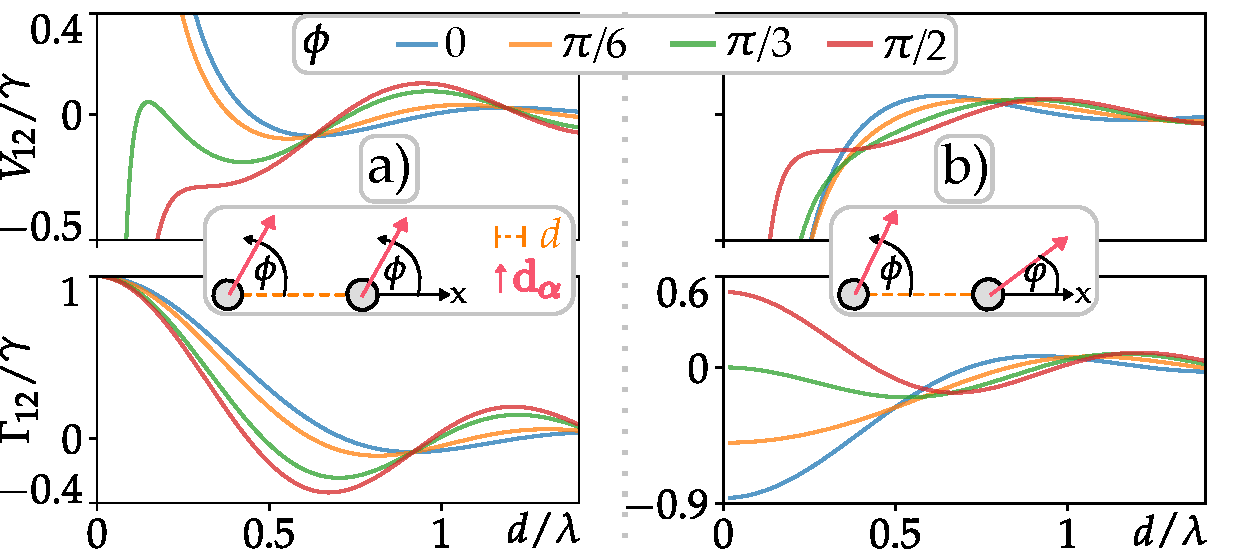
\includegraphics[width=0.8\textwidth]{2_atoms_Matrix_elems_combined(r)}
%    \decoRule
    \caption{The matrix element $ V_{12} $ and $ \Gamma_{12} $ represents the interaction strength between two atoms (dipole-dipole aswell as dissipation).
             They are plotted in units of $ \gamma $ against their separation $ d $ for different angles $ \phi $, which is measured with respect to the $x$-axis.
             \textbf{a)} Both dipoles are aligned.
             \textbf{b)} One dipole is fixed at $ \varphi = 5\pi/6 $ and one is varied.}
    \label{fig:N_2_Matrixemtry(r)}
\end{figure}

\noindent
To get closer to the desired setup, the number of atoms is now increased to $N = 3$.
The dipoles are assumed to lie within the plane defined by the resulting atomic triangle.
%as this is a physical approach.
This triangular configuration can be compared to the loop in \autoref{fig:botarellis_topo}.
The total phase \( \theta \)

\begin{equation}
    \theta \equiv \theta (\mathbf{r}_1, \mathbf{r}_2, \mathbf{r}_3, \mathbf{d}_1, \mathbf{d}_2, \mathbf{d}_3) \equiv  \Phi_{12} + \Phi_{23} + \Phi_{31},
\end{equation}

\noindent
can be defined, which represents the phase accumulated around the triangle.
To investigate the significance of $ \theta $, one can sum the three phases of Eq. \eqref{eq:phase_of_H_ab}
clockwise.
It turns out that when summing anticlockwise, the phase is the same, unlike in \autoref{Chapter3} (where the sign of $ \theta $ changes).
This is due to the Hamiltonian of the system being symmetric (and not Hermitian as in the work of Botarelli).
In addition,
it becomes evident, that different atomic separations and dipole orientations can add to the same phase $ \theta $.
This is shown in detail in \autoref{sec:No_direcionality} of the Appendix.

\noindent
In summary, it can be stated that, in contrast to the work of Botarelli, the phase $ \theta $ is not anymore the system-defining parameter.
The system of atoms is primarily characterised by the atomic separations and dipole orientations.

\noindent
While $ \theta $ is built up of these parameters, it does not provide the uniqueness of the system.
Different configurations add to the same $ \theta $,
and still result in distinct evolutions of the same excitation, contrary to \autoref{fig:The_Basis_evolution}.
In the following sections,
a condition will be introduced to still induce directional routing on the atomic system without the use of this phase.


%----------------------------------------------------------------------------------------
%	SECTION 2
%----------------------------------------------------------------------------------------
\section{Conditions for directional routing}\label{sec:solutions}
As described directional routing with atoms is not inherently possible by varying $\theta$.
However, one can achieve a controlled evolution by choosing specific dipole orientations and interatomic distances.
Without loss of generality, this work focuses on routing an excitation from the left into the upper arm.
Due to the system's symmetry along the $x$-axis, the results can be mirrored to achieve routing toward the lower arm as well.
To route an excitation into the upper arm, the matrix entries should satisfy the conditions

\begin{equation} \label{eq:Conditions}
\frac{V_{13}}{V_{12}} \ll 1 \quad \text{and} \quad \frac{V_{23}}{V_{12}} \ll 1 \text{.}
\end{equation}

\noindent
Here, the indices 1, 2 and 3 represent the atom of the triangle.
As described in \autoref{fig:N_2_Matrixemtry(r)}, changing the dipole orientation of different atoms modifies the elements $V_{\alpha \beta}$.
This modification can be helpful in meeting the conditions specified in Eq. \eqref{eq:Conditions}.
To explore this further, three topologies are investigated, illustrated in the upper part of \autoref{fig:Three_Topologies_and_optimization}.
%%Each of the systems will later be extended to configurations with $N > 6$ atoms.
For bigger systems,
additional atoms $N \geq 6$ are placed outside the triangle on extended lines between the center of the triangle
and the edge atoms.
The distances of these "outer" atoms are fixed at $d_\text{ext}$,
while the inner distance $d$ is varied.

\begin{figure}
    \centering
    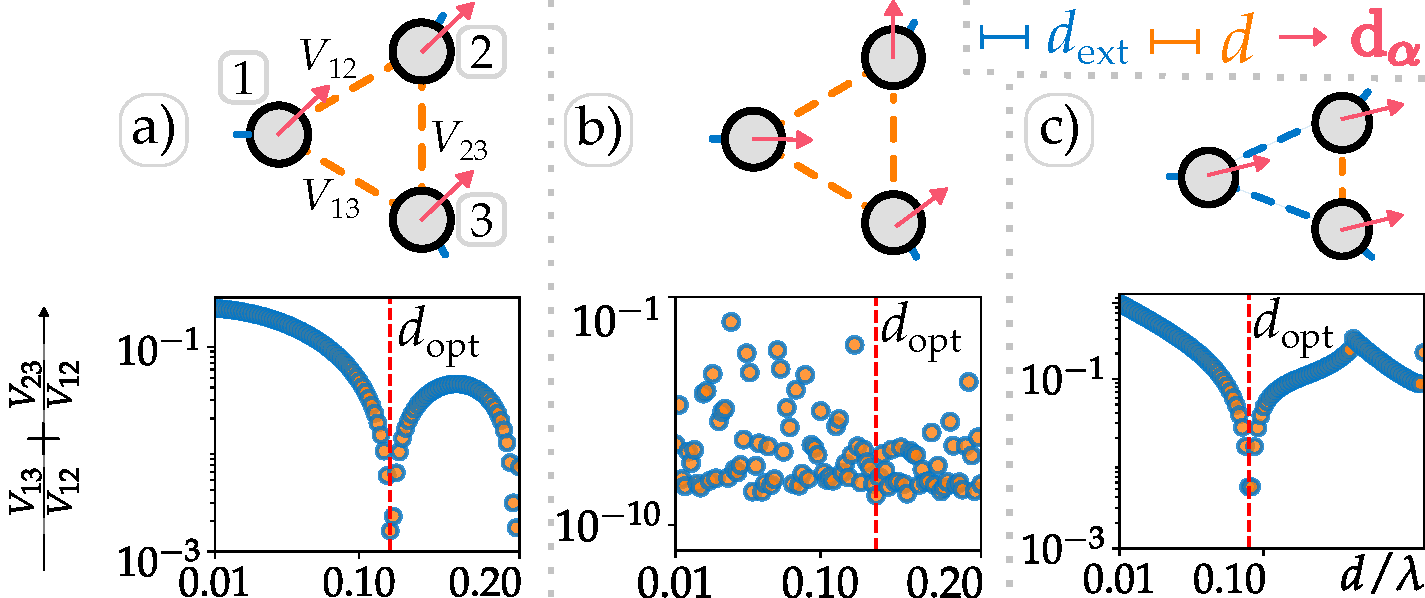
\includegraphics[width=0.8\textwidth]{Ratios_for2_Solutions}
%    \decoRule
    \caption{\textbf{a)} Equilateral triangle with aligned dipoles.
%    The dipoles are again measured with respect to the x-axis.
    \textbf{b)} Equilateral triangle with unique dipole orientations.
    \textbf{c)} Isosceles triangle, where one inner distance is changed and the dipoles are aligned.
    The dipole-dipole coupling strength $ V_{\alpha \beta} $ between each atom is indicated along the connection of two atoms.
    Each system will be investigated with $ N > 3 $ later, indicated by the small blue connections at each atom.
    \textbf{Conditions: }
    For each distance $ d $, there exists a set of dipole orientations,
        such that the ratios (Eq.
        \ref{eq:Conditions}) are minimal.
    % (measured with respect to the x-axis)
    The sum of these ratios is plotted with a logarithmic scaling against $ d $ in units of $\lambda$.
    Additionally, each topology offers one distance $ d_{\text{opt}} $, where the sum is minimal.
    An external distance of $ d_{\text{ext}} = 0.1 \lambda $ was used.}
    \label{fig:Three_Topologies_and_optimization}
\end{figure}

\noindent
The lower part of \autoref{fig:Three_Topologies_and_optimization} shows
that the two configurations with aligned dipoles (\textbf{a)} and \textbf{c)}) have a clear optimal distance, while
\textbf{b)} offers overall smaller values of the sum of both conditions in Eq. \eqref{eq:Conditions}.
It was separately checked that both conditions are small, and not just their sum.

\noindent
%For the Equilateral triangle, with aligned dipoles only 26\% and 66\% of the distances resulted in a setup,
%which satisfied the conditions with a threshold of \( 0.01 \).
In the completely symmetric system (\autoref{fig:Three_Topologies_and_optimization} \textbf{a)}), the optimal angle is \(\phi_{\text{opt}} = 30.04^\circ\) with an optimal distance of \(d_{\text{opt}} = 0.12\lambda\).
%When allowing unique dipoles, both conditions are satisfied 100\% of the time.
For case two (\textbf{b)}) the optimal angles are \(\phi_{\text{opt,1}} = 32.08^\circ\), \(\phi_{\text{opt,2}} = 29.63^\circ\), and \(\phi_{\text{opt,3}} = 29.12^\circ\), with an optimal distance of \(d_{\text{opt}} = 0.13\lambda\).
%When only one inner distance is varied, the conditions were only met 47\% and 55\% of the time.
For the isosceles triangle (\textbf{c)}), the optimal angle is \(\phi_{\text{opt}} = 31.69^\circ\) and the optimal distance is \(d_{\text{opt}} = 0.09\lambda\).
These values will be used in the subsequent analysis unless otherwise noted.



%-----------------------------------
%	SECTION 3
%-----------------------------------
\section{Implementation of Botarelli's system with six atoms}\label{subsec:botarellis_system}
With the optimal configurations identified,
the topology
proposed in Botarelli's paper \cite{Startingpoint} can be implemented with six atoms.
Using the just determined angles in the case of an equilateral triangle with aligned dipoles, the dipole of atom 2 is oriented directly towards atom 3.
This arrangement is visualized in \autoref{fig:EVO_System_with_atoms} \textbf{a)}.

\begin{figure}[!ht]
    \centering
    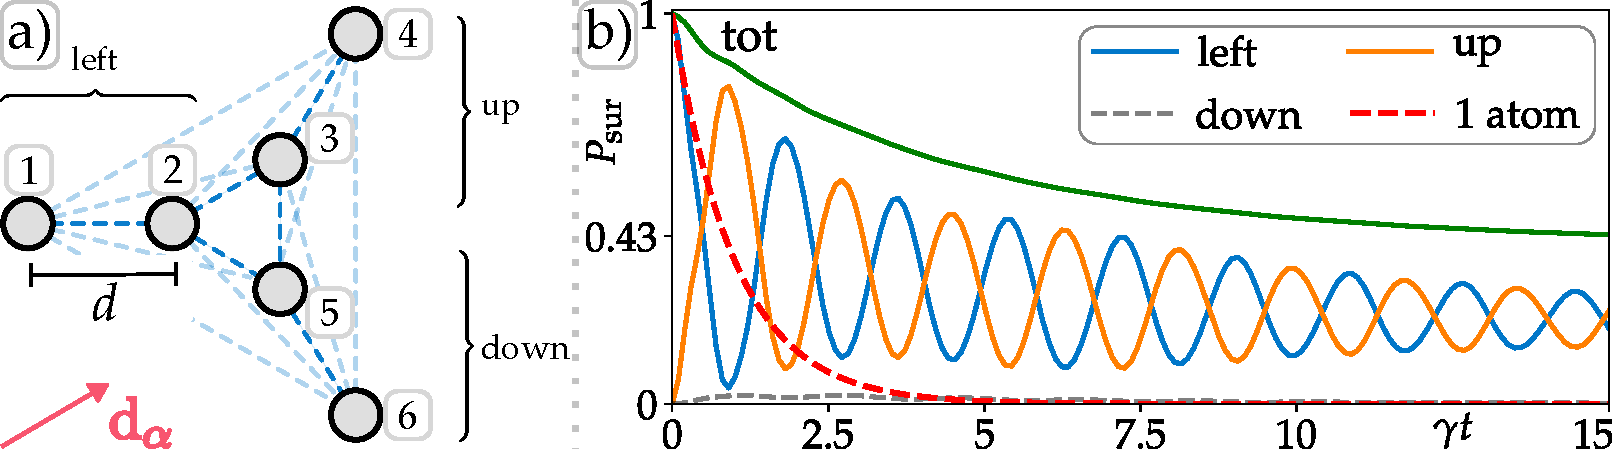
\includegraphics[width=1.0\textwidth]{System_with_atoms}
%    \decoRule
    \caption{\textbf{a)} A fully connected system of $N = 6$ atoms,
        which is maximally symmetric, mimicking the topology in \autoref{fig:botarellis_topo}.
    The dipole-dipole coupling strength $ V_{\alpha \beta} $ between each atom is indicated along the connection of two atoms.
    The opacity of a connection represents its strength, that depends on the distance between two atoms.
    The inner triangle is equilateral.
    All dipoles are  aligned indicated by $d_\alpha$.
    The system is initially in a superposition of atom 1 and 2 being excited.
    The state can mathematically be described by
    $ \vert \psi_x(0)\rangle =  \frac{1}{\sqrt{2}}\left[e^{i \varphi}, -e^{i \varphi}, 0, 0, 0, 0\right] \text{, with } \varphi \approx 1.3 $.\\ %2784
    \textbf{b)} Probability of finding the photonic excitation plotted against $ \gamma ^{-1}$.
    The total (\textbf{"tot"}) survival probability is displayed in green, while \textbf{"left"}
    means the probability of being on atoms (1,2), \textbf{"up"} refers to atoms (3,4), and
    \textbf{"down"} corresponds to atoms (5,6).
    As a reference, the red dashed line shows the single atomic behavior.}
    \label{fig:EVO_System_with_atoms}
\end{figure}

\noindent
Part \textbf{b)} shows the evolution of an initial state on the left arm.
The probability of finding the photon oscillates between the atoms (1,2) and (3,4).
The probability of being on atoms (5,6) is close to zero for all times.
\noindent
The lifetime of the photon being on the system is enhanced such that after $ T = 15 /\gamma $, the survival probability is $ 0.43$.
This can further be increased by using even more ($ N > 6 $) atoms \cite{AsenjoGarcia2017}.
This is why an initial state with a large number of atoms will now be defined.



%----------------------------------------------------------------------------------------
%	SUBSECTION 3
%----------------------------------------------------------------------------------------
\section{System definition with \texorpdfstring{$N > 6$}{N > 6}} \label{sec:Sys_def_N_bigger_6}
As discussed in section \ref{subsec:Phase_vel_Control},
the protocol for a given topology of $ N $ atoms in a specific arrangement with given dipole orientations is as follows.
First, the spectrum of the system is analyzed\footnote{The Hamiltonian of an infinite system can exactly be diagonalized with a Fourier transformation (FT).
For a finite systems, the diagonalization via a FT still holds only as an approximation (see \autoref{sec:Diagonalization} in the Appendix).
But, as discussed in \autoref{sec:K-space}, it is still useful to operate in quasi-momentum space.
}.

\noindent
In $k$-space, a Gaussian wave packet
\begin{equation}
    \vert \psi_k(t = 0) \rangle = (\sqrt{2 \pi}\sigma_k)^{-1/2} \sum_{i=1}^{N} e^{-(k-k_\text{s})^2/(4 \sigma_k^2)} \vert k_i \rangle
\end{equation}

\noindent
is initialized on a subradiant region ($\Gamma_k < 1$) with an approximately constant group velocity.
This wave packet has a peak at \( k_\text{s} \) with a width given by \( \sigma_k \).
The states $ \vert k_i \rangle $ are the $ N $ basis modes defined in \autoref{sec:K-space}.
%A phase multiplication is then applied to determine the center of the wave packet in real space.
%%e^{-i (\alpha - \nu)d_{\text{ext}}}
The state in real space can be obtained by applying the inverse Fourier transform (see Eq. \eqref{eq:FT}) to the state in $k$-space.
This resulting state maintains a Gaussian shape\footnote{Note that this relation strictly holds for an infinitely large system.
For finite systems, it should be treated with caution.
However, again, sufficiently large systems are considered here, so this relation can be used as a good approximation.} and is expressed as:

\begin{equation} \label{eq:Initial_state}
\vert \psi_x(t = 0) \rangle = \sqrt{\frac{\sigma_k}{\sqrt{2 \pi}}} \sum_{\alpha=1}^{N} e^{-i k_\text{s} \overbrace{(\alpha - \nu)d_{\text{ext}}}^{\mathbf{r}_{\alpha-\nu}}} e^{-(\alpha - \nu)^2 d_{\text{ext}}^2\sigma_k^2} \vert e_\alpha \rangle \equiv \sum_{\alpha=1}^{N} c_{\alpha}(0) \vert e_\alpha \rangle.
\end{equation}

\noindent
In this expression, \( \nu \) represents the atom index where the Gaussian has its peak.
The parameter \( d_\text{ext} \) denotes the atomic separation in the chain and
\( \vert e_\alpha \rangle \) (a real-space basis state) refers to the \( \alpha \)-th atom being excited.

%----------------------------------------------------------------------------------------
%	SUBSECTION 3.1
%----------------------------------------------------------------------------------------
\subsection{Transport}
The protocol for defining the initial state given by Eq. \eqref{eq:Initial_state} and its evolution is illustrated for a finite one-dimensional chain of $ N = 100 $ atoms in \autoref{fig:MOM_REAL_SPACE_CHAIN}.
\begin{figure}
    \centering
    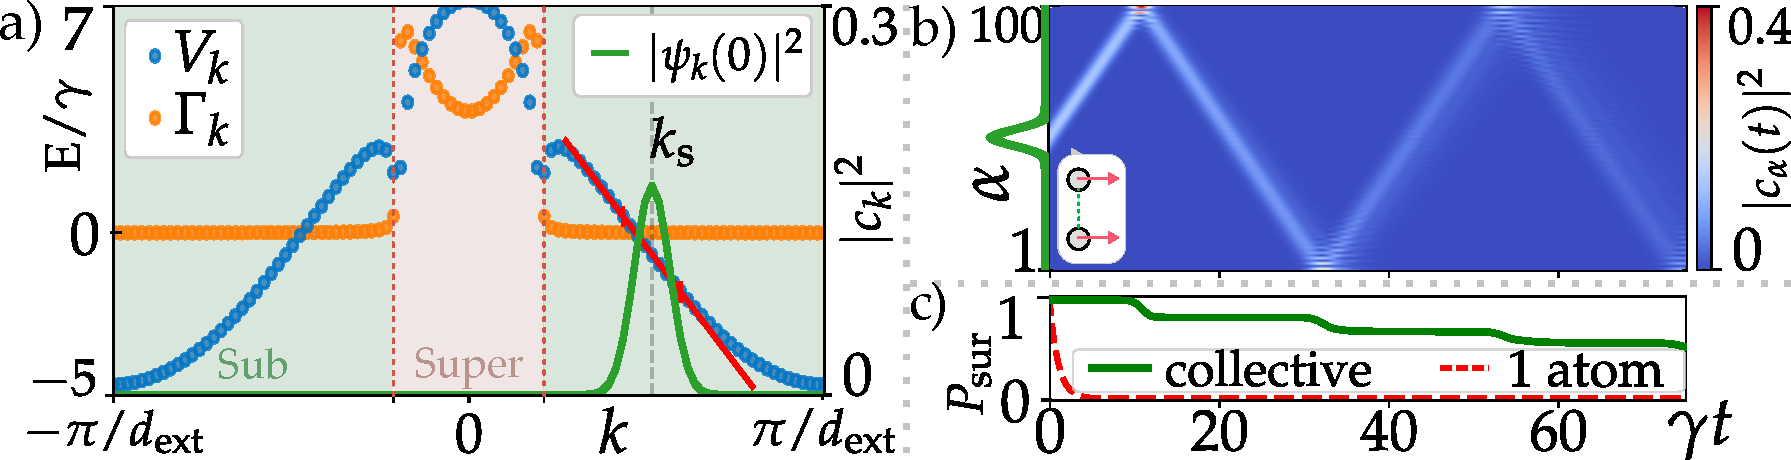
\includegraphics[width=1.0\textwidth]{CHAIN_MOM_EVO}
%    \decoRule
    \caption{The dipoles are perpendicular to the chain of $N= 100$ atoms.
    \textbf{a)} Spectrum ($ V_k $), Eigen-Decay modes ($ \Gamma_k $) and norm of the wave packet $ |\psi_k(0)|^2 $ in momentum space are plotted against the pseudo momentum $k$.
    The regions of sub- and superradiance ($ \Gamma_k < 1 \text{ and } > 1$) are shaded in green and red respectively.
    Here an interatomic distance of $ d_\text{ext} = 0.1 \lambda$ was used.
    The wave packet in $k$-space has a width of $ \sigma_k = 0.05 \frac{\pi}{d_\text{ext}} $  around $ k_\text{s} \approx 0.5 \frac{\pi}{d_\text{ext}} $.
    A straight (red line) has been fitted through to modes $ V_k $ over a range $[k_\text{s} \pm 2\sigma_k]$
        indicating a linear regime in $ V_k $.
    \textbf{b)} The initial state$ \vert \psi_x(t = 0) \rangle $,
        depicted as a green line left of the color plot is evolved.
        The probability of being on the $ \alpha $-th atom against time is plotted in units of $ \gamma^{-1}$.
    \textbf{c)} The survival probability is plotted against time in units of $\gamma^{-1}$.
        The green line indicates the total, collective survival probability,
        and the dashed red line indicates the single atom decay as a reference.}
    \label{fig:MOM_REAL_SPACE_CHAIN}
\end{figure}

\noindent
The wave packet is reflected at the chain end and slightly disperses.
When this happens, the survival probability is significantly reduced.
For the evolution in the bulk, the survival probability stays approximately constant with time.

\noindent
In the topology of interest, the $ N $ atoms are arranged into three distinct chains shown in \autoref{fig:Setup_all_inner_distances}.
The left chain (left) consists of atoms numbered from 1 to \( N/3  \),
the upper chain (up) comprises atoms numbered from \(  N/3  + 1 \) to \(  2N/3  \),
and the lower chain (down) includes the remaining atoms from \( 2N/3  + 1 \) to \( N \).
For the case of unique dipoles, the atoms on the left, up and down chain all have their own dipole angle $ \phi_{\text{opt,1,2,3}} $ respectively.
Within the chain, they are aligned.
The wave packet will only be initialized on the left chain.
All coefficients $ c_\alpha: { N/3 < \alpha \leq N} $ of the state $ \vert \psi_x(t = 0) \rangle $ are set to zero.

\begin{figure}[!ht]
    \centering
    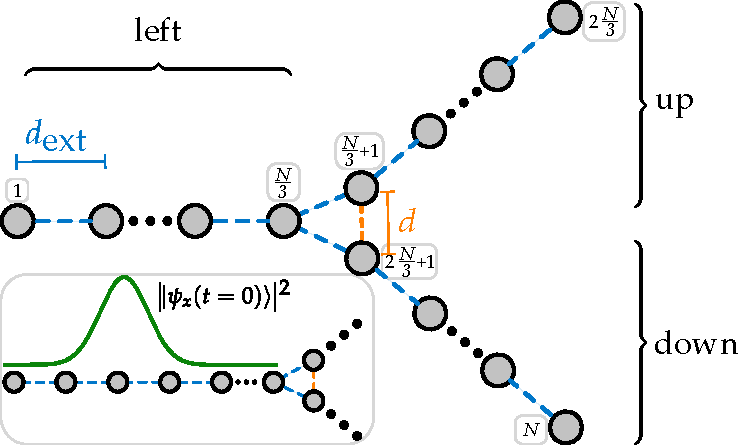
\includegraphics[width=0.75\textwidth]{system_1_inner}
    \caption{Setup for $N$ atoms with an isosceles inner triangle.
    The initial state is a Gaussian, localized near the center of the left arm as indicated by the green line.
    Full connectivity is omitted for visual clarity, although every atom interacts with every other atom.
    A similar arrangement can be made with an equilateral triangle.}
    \label{fig:Setup_all_inner_distances}
\end{figure}

\noindent
The same protocol applied to a single chain can be used here.
The shape of the spectrum depends on both the atomic distance and the dipole orientations of the left chain.
Three systems with $N$ atoms and the inner triangles according to \autoref{fig:MOM_REAL_SPACE_CHAIN} \textbf{a)},\textbf{b)} and \textbf{c)}
are used.
For cases \textbf{a)} and \textbf{b)}, the optimal inner distance is used for the external distance as well.
In contrast, with case \textbf{c)} an external distance of  $ d_\text{ext} = 0.1 \lambda $ is used.
Generally, the group velocity in the subradiant regime increases as the atomic distance in the chain decreases,
Therefore, a smaller choice of \( d_\text{ext} \) results in a faster propagation of the wave packet along the chain, allowing it to reach the inner triangle more quickly.

\noindent
When the wave packet encounters the triangle, a transmission ($T$), reflection ($R$), and a small leakage ($L$) are expected.
%, since perfect coupling cannot be achieved.
These coefficients can be defined as
\begin{equation}
    T = \frac{P_{\text{up}(t=T)}}{P_{\text{left}(t=0)}} \text{,} \quad R = \frac{P_{\text{left}(t=T)}}{P_{\text{left}(t=0)}} \quad \text{and} \quad L = \frac{P_{\text{down}(t=T)}}{P_{\text{left}(t=0)}}\text{.}
\end{equation}

\newpage
\noindent
Here, \(t=T\) represents a point in time after the routing event when each part of the original wave packet is far away from the triangle.
With this, one can measure the effectiveness of routing in the different topologies.


    %----------------------------------------------------------------------------------------
%	SECTION 4
%----------------------------------------------------------------------------------------
\newpage
\section{Routing in systems with \texorpdfstring{$N = 60$}{N = 60} atoms}
Starting from $N = 60$ a wave packet that does not couple to any superradiant modes and has a well-defined center in real space can be initialized on the system.
The evolutions for this case are shown in \autoref{fig:EVO_Topologies_N_60}.
\begin{figure}[!ht]
    \centering
    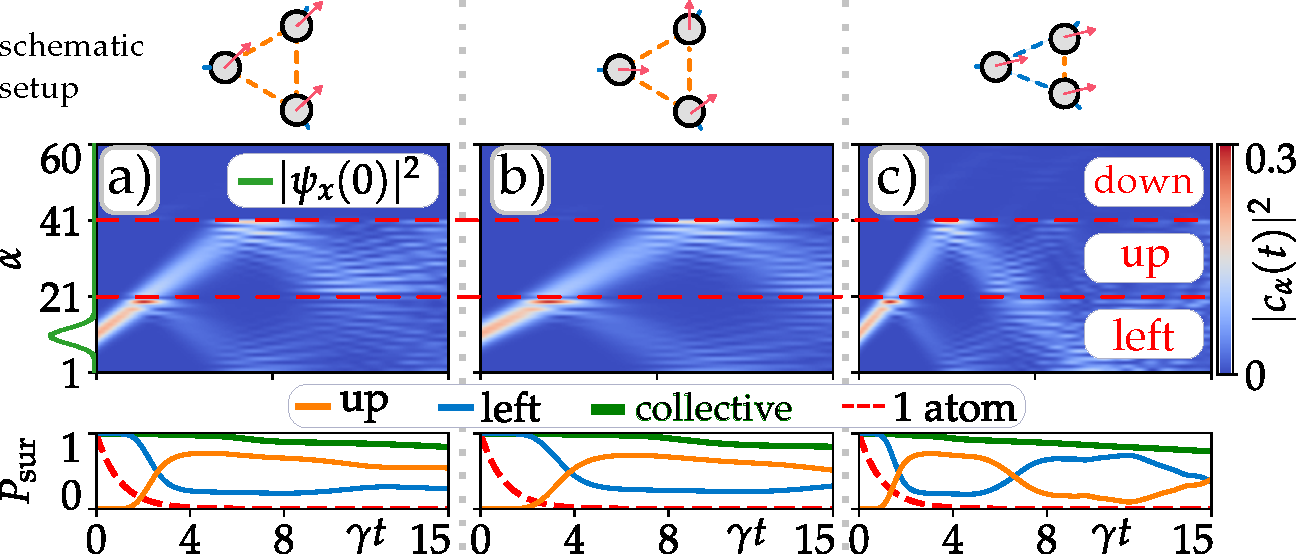
\includegraphics[width=0.8\textwidth]{Topologies_EVO_N_60}
%    \decoRule
    \caption{System with $N = 60$ atoms.
    \textbf{a)} Equilateral triangle with aligned dipoles.
    \textbf{b)} Equilateral triangle with unique dipoles.
    \textbf{c)} Isosceles triangle with aligned dipoles.
    For each system, the same initial state$ \vert \psi_x(t = 0) \rangle $,
    depicted as a green line left of the first color plot is evolved.
    The optimal setups (see section
    \ref{sec:solutions}) are used, with $\sigma_k = 0.08 \frac{\pi}{d_\text{ext}}$ and $k_\text{s} \approx 0.58 \frac{\pi}{d_\text{ext}}$.
    The probability of being on the $ \alpha $-th atom against time is plotted in units of $ \gamma^{-1}$.
    The lower plots show the survival probability (\textbf{"tot"} in green, \textbf{"left"} and \textbf{"up"} shows the probability
        of finding the photonic excitation on the atoms of the left and upper chain respectively.
    This time \textbf{"down"} is not shown.
    As a reference, the red-dashed line shows the single atomic behavior.}
    \label{fig:EVO_Topologies_N_60}
\end{figure}


\noindent
In this minimal example, the survival probability after $T = 15 /\gamma$ is $0.82$, $0.83$
and $0.77$ for topologies \textbf{a)}, \textbf{b)} and \textbf{c)} respectively.
In comparison to $ 6 $ atoms, the survival probability increases by nearly 100 percent.
An observable dispersion occurs indicating that a larger atomic number is necessary to achieve more robust routing.
Table \ref{tab:coefficients_N_60} presents the reflection, transmission, and leakage coefficients for the three topologies.

\begin{table}[h!]
    \centering
    \caption{Reflection $R$, transmission $T$, and leakage $L$ coefficients for three topologies with $N = 60$.
    Here, "E" stands for equilateral geometry, and "I"
    stands for isosceles geometry and "aligned" ("unique") hints at the dipole orientations.}
    \begin{tabular}{@{}lccc@{}}
        \toprule
        \textbf{Case} & \textbf{$ R $} & \textbf{$ T $} & \textbf{$ L $} \\
        \midrule
        E, aligned ($T = 4 / \gamma$) & 22.97 & 73.99 & 1.01 \\
        E, unique ($T = 6 / \gamma$)    & 25.68 & 71.59 & 0.46 \\
        I, aligned ($T = 3 / \gamma$)   & 20.38 & 73.73 & 2.82 \\
        \bottomrule
    \end{tabular}
    \label{tab:coefficients_N_60}
\end{table}

\noindent
As shown in Table~\ref{tab:coefficients_N_60}, the reflection and transmission coefficients vary slightly across the cases.
The data is collected at different time points, because the group velocity is different for each case.
The equilateral topology with unique dipoles has the highest reflection coefficient, while the totally symmetric (equilateral, aligned) and isosceles topologies exhibit slightly higher transmission.
Leakage into the lower arm remains relatively small across all configurations, with the isosceles topology showing the highest leakage of $L = 2.82$.
Overall, these results suggest that while the equilateral triangle with unique dipoles can maximize reflection, other configurations might offer a better transmission control.
Since the three cases have slightly different interatomic distances \( d_\text{ext} \),
the group velocity changes.
This results in the fastest transmission for the isosceles case and the slowest for the equilateral case with unique dipoles.

\noindent
At equal external distances of $ 0.1 \lambda $,
only small deviations are expected to stem from the different dipole orientations on the chains.
That is why this case is not explicitly shown.




%----------------------------------------------------------------------------------------
%	SECTION 4
%----------------------------------------------------------------------------------------
\section{Routing in systems with \texorpdfstring{$N = 300$}{N = 300} atoms} \label{sec:N_300}
As discussed, the dispersion is expected to decrease for more atoms.
To investigate the effect, $ N $ is increased by a factor of 5.

\noindent
Previously, the interatomic distance was manipulated to affect the transmission, which already resulted in changes to the group velocity and motivates the following discussion.
Now, the focus shifts to investigating the initial wave packet itself.
In particular, the effect of $k_s$ (the center of the wave packet in $k$-space) on the transmission is analyzed.

\noindent
In the equilateral triangle with unique dipoles, the coupling ratios are very small for many distances within the studied range.
For example, the distance $d = 0.05 \lambda \neq d_{\text{opt}}$ of the three inner atoms also fulfills the conditions Eq. \eqref{eq:Conditions} very good.
This distance, as well as $d_\text{ext} = 0.05 \lambda $, which results in a faster propagation of the wave packet along the chain, is chosen for the following analysis.

\begin{figure}[!ht]
    \centering
    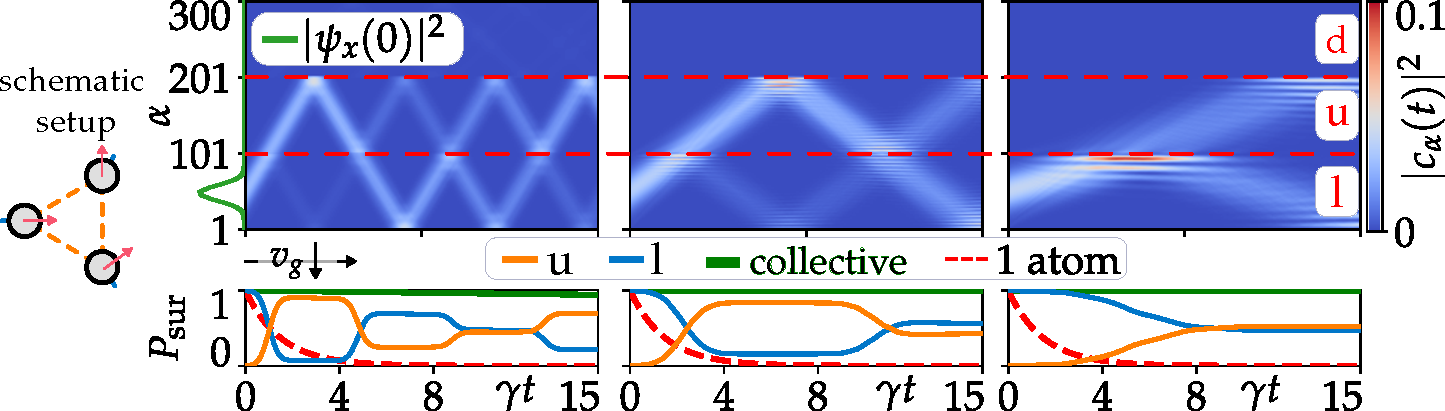
\includegraphics[width=1.0\textwidth]{Topologies_EVO_N_300_v_g}
%    \decoRule
    \caption{Evolution for a system with $ N = 300 $ and an equilateral triangle with unique dipoles.
    The distance is chosen to be \(d \approx 0.05 \lambda \) and the corresponding angles \( \phi_{1,2,3} = [22.12^\circ, 38.56^\circ, 29.68^\circ] \) are extracted from \autoref{fig:Three_Topologies_and_optimization}.
    The same quantities as in \autoref{fig:EVO_Topologies_N_60} are plotted for different initial states.
    The wave packet is centered around $k_\text{s} = 0.43, 0.79, 0.92 \frac{\pi}{d_\text{ext}} $ from left to right and $ \sigma_k = 0.01 \frac{\pi}{d_\text{ext}} $.
    Increasing $k_\text{s}$ reduces the group velocity $ v_\text{g} $.}
    \label{fig:Routing_dep_on_v_g}
\end{figure}

\noindent
As can be seen in \autoref{fig:Routing_dep_on_v_g}, a higher group velocity results in a higher transmission $T$.
As $ k_\text{s} $ increases,
the group velocity $ v_\text{g} $ decreases because the dispersion is less steep at the Brillouin zone boundary $ k = \pm \frac{\pi}{d_\text{ext}} $ (see \autoref{fig:MOM_REAL_SPACE_CHAIN}).
%Generally using a bigger $ k_s $,
%closer to the Brillouin zone boundary $ k = \pm \frac{\pi}{d_\text{ext}} $ results in a smaller group velocity,
%because the dispersion is steeper at the Brillouin zone center.
As a result, the transmission decreases.
However, a higher group velocity and thus higher transmission comes at the cost of a higher dissipation,
which can be seen
since the collective survival probability $P_{\text{sur}}$ decreases faster for lower $ k_{\text{s}}$.
This observation aligns with the fact that the Brillouin zone center corresponds to the superradiant regime (see \autoref{fig:MOM_REAL_SPACE_CHAIN}).

\begin{table}[h!]
\centering
\caption{The dependence of $ k_\text{s} $ on $R$, $T$, and $L$ for $N = 300$ and an equilateral triangle with unique dipoles}
\begin{tabular}{@{}cc@{}}
    % Subfigure containing the figure on the left
    \begin{minipage}{0.22\textwidth}
        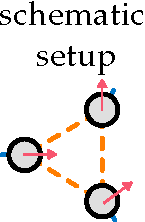
\includegraphics[width=0.5\textwidth]{Topologie_SETUP_N_300_v_g}
    \end{minipage} &
    % The table on the right
    \begin{minipage}{0.78\textwidth}
        \begin{tabular}{@{}lccc@{}}
        \toprule
        \textbf{Case} & \textbf{$ R $} & \textbf{$ T $} & \textbf{$ L $} \\
        \midrule
        \textbf{$k_\text{s} = 0.43 \frac{\pi}{d_\text{ext}}$ ($T = 1 / \gamma$)} & 8.58 & 89.28 & 1.92 \\
        \textbf{$k_\text{s} = 0.79 \frac{\pi}{d_\text{ext}}$ ($T = 3 / \gamma$)} & 15.73 & 84.02 & 0.00 \\
        \textbf{$k_\text{s} = 0.92 \frac{\pi}{d_\text{ext}}$ ($T = 7 / \gamma$)} & 47.62 & 52.28 & 0.00 \\
        \bottomrule
        \end{tabular}
    \end{minipage}
\end{tabular}
\label{tab:coefficients_k_s}
\end{table}

\noindent
Table \ref{tab:coefficients_k_s} presents the reflection, transmission, and leakage coefficients for varying values of $k_\text{s}$.
As $k_\text{s}$ increases, the reflection coefficient ($R$) also increases, while the transmission coefficient ($T$) decreases.
This indicates that a higher group velocity, associated with smaller $k_\text{s}$ favors transmission.

\vspace{1cm}
\noindent
The symmetric topology, the equilateral triangle with unique dipoles, and isosceles triangle, have provided a comprehensive understanding of how the group velocity, atomic distance, and dipole orientations influence the transmission.

\noindent
Having analyzed all factors
that determine the transmission of a photonic excitation on the system of three connected atomic chains,
the overall optimized conditions will now be applied for $N = 300$ atoms.
Therefore, the optimal configurations of the three topologies
as well as the center of the wave packet $ k_{\text{s}}$ are chosen as a balance between low dissipation, robust and fast propagation.
The results are visualized in \autoref{fig:EVO_Topologies}.

\begin{figure}[!ht]
    \centering
    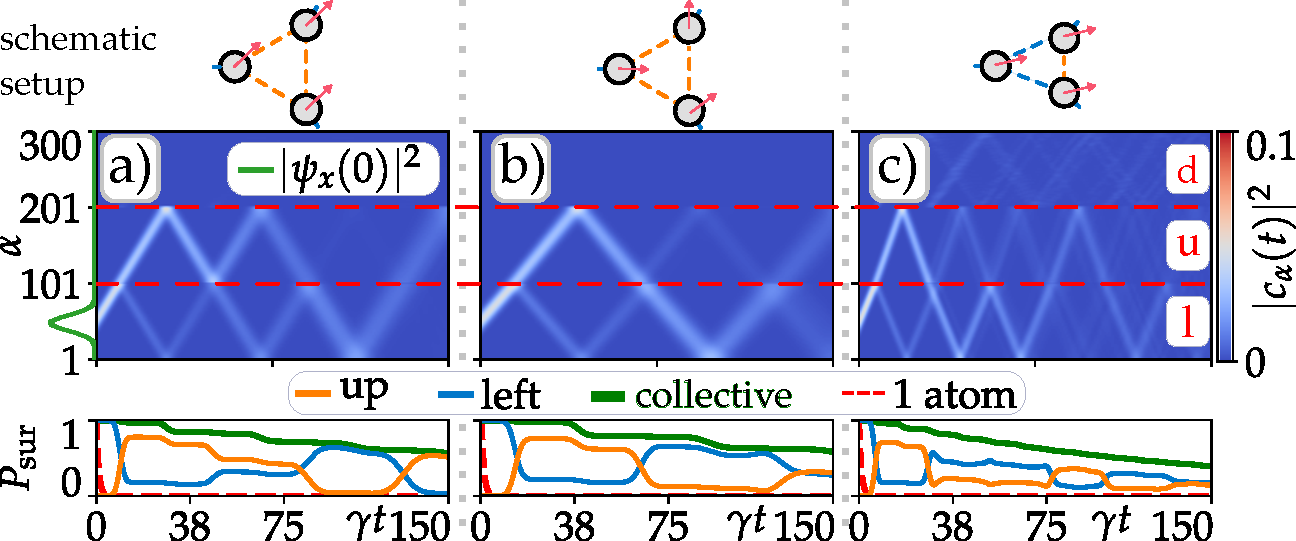
\includegraphics[width=0.8\textwidth]{Topologies_EVO_N_300_final}
    \caption{Evolution for $ N = 300 $ with $ \sigma_k = 0.02 \frac{\pi}{d_\text{ext}} $ and  $k_\text{s} \approx 0.5 \frac{\pi}{d_\text{ext}} $.
    This figure shows similar plots as in Fig.~\ref{fig:EVO_Topologies_N_60}, now for the optimal configurations of \autoref{sec:solutions}:
    \textbf{a)} Symmetric topology with \(\phi_{\text{opt}} = 30.04^\circ\), \(d_{\text{opt}} = 0.12\lambda\), \textbf{b)} Equilateral triangle with unique dipoles \(\phi_{\text{opt,1}} = 32.08^\circ\), \(\phi_{\text{opt,2}} = 29.63^\circ\) and \(\phi_{\text{opt,3}} = 29.12^\circ\), \(d_{\text{opt}} = 0.13\lambda\) and \textbf{c)} Isosceles triangle with aligned dipoles with \(\phi_{\text{opt}} = 31.69^\circ\) and \(d_{\text{opt}} = 0.09\lambda\).}
    \label{fig:EVO_Topologies}
\end{figure}


\noindent
For all triangle types, the wave packet primarily transmits into the upper arm, with variations in reflection into the left arm and leakage into the lower arm.
The reflection ($R$), transmission ($T$), and leakage ($L$) coefficients for each setup are highlighted in \autoref{tab:coefficients_topologies}

\begin{table}[h!]
\centering
\caption{Reflection ($R$), Transmission ($T$), and Leakage ($L$) coefficients for different topologies with $N = 300$ at $k_\text{s} \approx 0.5 \frac{\pi}{d_\text{ext}} $.
    Again, "E" means equilateral geometry, and "I"
    stands for isosceles geometry while "aligned" ("unique") hints at the dipole orientations.}
\begin{tabular}{@{}lccc@{}}
    \toprule
    \textbf{Topology} & \textbf{$R$} & \textbf{$T$} & \textbf{$L$} \\
    \midrule
    E, aligned ($T = 20 / \gamma$) & 17.84 & 78.22 & 1.17 \\
    E, unique ($T = 20 / \gamma$) & 22.30 & 75.68 & 0.04 \\
    I, ligned ($T = 15 / \gamma$) & 17.90 & 70.77 & 7.49 \\
    \bottomrule
\end{tabular}
\label{tab:coefficients_topologies}
\end{table}

\noindent
The equilateral triangle generally exhibits higher transmission and lower reflection compared to the isosceles triangle, with minimal leakage.
In the equilateral triangle, the wave packet components that split at the triangle effectively overlap when they encounter the triangle again.
This results in a more consistent group velocity along each chain, enhancing overall transmission and reducing leakage.
Each encounter with a chain's edge results in a small dip in survival probability, similar to a single chain scenario.
For the isosceles triangle, these dips occur more frequently, reducing the survival probability over time.
The smaller atomic distances of the chain $ d_\text{ext} $ in this topology increase the group velocity, leading to more reflections and consequently higher losses.
This results in the lowest survival probability among the topologies studied, with notable leakage into the lower arm.
The completely symmetric topology demonstrates the highest stability, with no significant leakage and a relatively high transmission coefficient.
The setup with unique dipole orientations offers similarly good results.
However, it is not physically achievable in practice.
Therefore, the equilateral triangle with aligned dipoles is more relevant for stable readout.
The isosceles triangle is suitable for faster readout at the cost of an increased leakage.